
%% bare_jrnl.tex
%% V1.3
%% 2007/01/11
%% by Michael Shell
%% see http://www.michaelshell.org/
%% for current contact information.
%%
%% This is a skeleton file demonstrating the use of IEEEtran.cls
%% (requires IEEEtran.cls version 1.7 or later) with an IEEE journal paper.
%%
%% Support sites:
%% http://www.michaelshell.org/tex/ieeetran/
%% http://www.ctan.org/tex-archive/macros/latex/contrib/IEEEtran/
%% and
%% http://www.ieee.org/


% *** Authors should verify (and, if needed, correct) their LaTeX system  ***
% *** with the testflow diagnostic prior to trusting their LaTeX platform ***
% *** with production work. IEEE's font choices can trigger bugs that do  ***
% *** not appear when using other class files.                            ***
% The testflow support page is at:
% http://www.michaelshell.org/tex/testflow/


%%*************************************************************************
%% Legal Notice:
%% This code is offered as-is without any warranty either expressed or
%% implied; without even the implied warranty of MERCHANTABILITY or
%% FITNESS FOR A PARTICULAR PURPOSE! 
%% User assumes all risk.
%% In no event shall IEEE or any contributor to this code be liable for
%% any damages or losses, including, but not limited to, incidental,
%% consequential, or any other damages, resulting from the use or misuse
%% of any information contained here.
%%
%% All comments are the opinions of their respective authors and are not
%% necessarily endorsed by the IEEE.
%%
%% This work is distributed under the LaTeX Project Public License (LPPL)
%% ( http://www.latex-project.org/ ) version 1.3, and may be freely used,
%% distributed and modified. A copy of the LPPL, version 1.3, is included
%% in the base LaTeX documentation of all distributions of LaTeX released
%% 2003/12/01 or later.
%% Retain all contribution notices and credits.
%% ** Modified files should be clearly indicated as such, including  **
%% ** renaming them and changing author support contact information. **
%%
%% File list of work: IEEEtran.cls, IEEEtran_HOWTO.pdf, bare_adv.tex,
%%                    bare_conf.tex, bare_jrnl.tex, bare_jrnl_compsoc.tex
%%*************************************************************************

% Note that the a4paper option is mainly intended so that authors in
% countries using A4 can easily print to A4 and see how their papers will
% look in print - the typesetting of the document will not typically be
% affected with changes in paper size (but the bottom and side margins will).
% Use the testflow package mentioned above to verify correct handling of
% both paper sizes by the user's LaTeX system.
%
% Also note that the "draftcls" or "draftclsnofoot", not "draft", option
% should be used if it is desired that the figures are to be displayed in
% draft mode.
%
%\documentclass[conference]{IEEEtran}
\documentclass[12pt,journal,compsoc]{IEEEtran}

%
% If IEEEtran.cls has not been installed into the LaTeX system files,
% manually specify the path to it like:
% \documentclass[journal]{../sty/IEEEtran}





% Some very useful LaTeX packages include:
% (uncomment the ones you want to load)


% *** MISC UTILITY PACKAGES ***
%
%\usepackage{ifpdf}
% Heiko Oberdiek's ifpdf.sty is very useful if you need conditional
% compilation based on whether the output is pdf or dvi.
% usage:
% \ifpdf
%   % pdf code
% \else
%   % dvi code
% \fi
% The latest version of ifpdf.sty can be obtained from:
% http://www.ctan.org/tex-archive/macros/latex/contrib/oberdiek/
% Also, note that IEEEtran.cls V1.7 and later provides a builtin
% \ifCLASSINFOpdf conditional that works the same way.
% When switching from latex to pdflatex and vice-versa, the compiler may
% have to be run twice to clear warning/error messages.



\usepackage{listings}
\usepackage{enumerate}
\usepackage{array}
\usepackage{url}

\makeatletter
\newcommand\thefontsize[1]{}
\makeatother


\lstloadlanguages{Python}
%\usepackage{amsmath}

% *** CITATION PACKAGES ***
%
\usepackage{cite}
% cite.sty was written by Donald Arseneau
% V1.6 and later of IEEEtran pre-defines the format of the cite.sty package
% \cite{} output to follow that of IEEE. Loading the cite package will
% result in citation numbers being automatically sorted and properly
% "compressed/ranged". e.g., [1], [9], [2], [7], [5], [6] without using
% cite.sty will become [1], [2], [5]--[7], [9] using cite.sty. cite.sty's
% \cite will automatically add leading space, if needed. Use cite.sty's
% noadjust option (cite.sty V3.8 and later) if you want to turn this off.
% cite.sty is already installed on most LaTeX systems. Be sure and use
% version 4.0 (2003-05-27) and later if using hyperref.sty. cite.sty does
% not currently provide for hyperlinked citations.
% The latest version can be obtained at:
% http://www.ctan.org/tex-archive/macros/latex/contrib/cite/
% The documentation is contained in the cite.sty file itself.






% *** GRAPHICS RELATED PACKAGES ***
%
\ifCLASSINFOpdf
  \usepackage[pdftex]{graphicx}
  % declare the path(s) where your graphic files are
  \graphicspath{{../pdf/}{../jpeg/}}
  % and their extensions so you won't have to specify these with
  % every instance of \includegraphics
  \DeclareGraphicsExtensions{.pdf,.jpeg,.png, .PNG, .GIF}
\else
  % or other class option (dvipsone, dvipdf, if not using dvips). graphicx
  % will default to the driver specified in the system graphics.cfg if no
  % driver is specified.
  \usepackage[dvips]{graphicx}
  % declare the path(s) where your graphic files are
  \graphicspath{{../eps/}}
  % and their extensions so you won't have to specify these with
  % every instance of \includegraphics
  \DeclareGraphicsExtensions{.eps}
\fi
% graphicx was written by David Carlisle and Sebastian Rahtz. It is
% required if you want graphics, photos, etc. graphicx.sty is already
% installed on most LaTeX systems. The latest version and documentation can
% be obtained at: 
% http://www.ctan.org/tex-archive/macros/latex/required/graphics/
% Another good source of documentation is "Using Imported Graphics in
% LaTeX2e" by Keith Reckdahl which can be found as epslatex.ps or
% epslatex.pdf at: http://www.ctan.org/tex-archive/info/
%
% latex, and pdflatex in dvi mode, support graphics in encapsulated
% postscript (.eps) format. pdflatex in pdf mode supports graphics
% in .pdf, .jpeg, .png and .mps (metapost) formats. Users should ensure
% that all non-photo figures use a vector format (.eps, .pdf, .mps) and
% not a bitmapped formats (.jpeg, .png). IEEE frowns on bitmapped formats
% which can result in "jaggedy"/blurry rendering of lines and letters as
% well as large increases in file sizes.
%
% You can find documentation about the pdfTeX application at:
% http://www.tug.org/applications/pdftex





% *** MATH PACKAGES ***
%
\usepackage[cmex10]{amsmath}
% A popular package from the American Mathematical Society that provides
% many useful and powerful commands for dealing with mathematics. If using
% it, be sure to load this package with the cmex10 option to ensure that
% only type 1 fonts will utilized at all point sizes. Without this option,
% it is possible that some math symbols, particularly those within
% footnotes, will be rendered in bitmap form which will result in a
% document that can not be IEEE Xplore compliant!
%
% Also, note that the amsmath package sets \interdisplaylinepenalty to 10000
% thus preventing page breaks from occurring within multiline equations. Use:
\interdisplaylinepenalty=2500
% after loading amsmath to restore such page breaks as IEEEtran.cls normally
% does. amsmath.sty is already installed on most LaTeX systems. The latest
% version and documentation can be obtained at:
% http://www.ctan.org/tex-archive/macros/latex/required/amslatex/math/





% *** SPECIALIZED LIST PACKAGES ***
%
\usepackage{algorithm}
\usepackage{algorithmic}
\renewcommand{\algorithmicrequire}{\textbf{Input:}}
\renewcommand{\algorithmicensure}{\textbf{Output:}}
%\usepackage[noend]{algpseudocode}
% algorithmic.sty was written by Peter Williams and Rogerio Brito.
% This package provides an algorithmic environment fo describing algorithms.
% You can use the algorithmic environment in-text or within a figure
% environment to provide for a floating algorithm. Do NOT use the algorithm
% floating environment provided by algorithm.sty (by the same authors) or
% algorithm2e.sty (by Christophe Fiorio) as IEEE does not use dedicated
% algorithm float types and packages that provide these will not provide
% correct IEEE style captions. The latest version and documentation of
% algorithmic.sty can be obtained at:
% http://www.ctan.org/tex-archive/macros/latex/contrib/algorithms/
% There is also a support site at:
% http://algorithms.berlios.de/index.html
% Also of interest may be the (relatively newer and more customizable)
% algorithmicx.sty package by Szasz Janos:
% http://www.ctan.org/tex-archive/macros/latex/contrib/algorithmicx/




% *** ALIGNMENT PACKAGES ***
%
%\usepackage{array}
% Frank Mittelbach's and David Carlisle's array.sty patches and improves
% the standard LaTeX2e array and tabular environments to provide better
% appearance and additional user controls. As the default LaTeX2e table
% generation code is lacking to the point of almost being broken with
% respect to the quality of the end results, all users are strongly
% advised to use an enhanced (at the very least that provided by array.sty)
% set of table tools. array.sty is already installed on most systems. The
% latest version and documentation can be obtained at:
% http://www.ctan.org/tex-archive/macros/latex/required/tools/


%\usepackage{mdwmath}
%\usepackage{mdwtab}
% Also highly recommended is Mark Wooding's extremely powerful MDW tools,
% especially mdwmath.sty and mdwtab.sty which are used to format equations
% and tables, respectively. The MDWtools set is already installed on most
% LaTeX systems. The lastest version and documentation is available at:
% http://www.ctan.org/tex-archive/macros/latex/contrib/mdwtools/


% IEEEtran contains the IEEEeqnarray family of commands that can be used to
% generate multiline equations as well as matrices, tables, etc., of high
% quality.


%\usepackage{eqparbox}
% Also of notable interest is Scott Pakin's eqparbox package for creating
% (automatically sized) equal width boxes - aka "natural width parboxes".
% Available at:
% http://www.ctan.org/tex-archive/macros/latex/contrib/eqparbox/





% *** SUBFIGURE PACKAGES ***
%\usepackage[tight,footnotesize]{subfigure}
% subfigure.sty was written by Steven Douglas Cochran. This package makes it
% easy to put subfigures in your figures. e.g., "Figure 1a and 1b". For IEEE
% work, it is a good idea to load it with the tight package option to reduce
% the amount of white space around the subfigures. subfigure.sty is already
% installed on most LaTeX systems. The latest version and documentation can
% be obtained at:
% http://www.ctan.org/tex-archive/obsolete/macros/latex/contrib/subfigure/
% subfigure.sty has been superceeded by subfig.sty.



%\usepackage[caption=false]{caption}
%\usepackage[font=footnotesize]{subfig}
% subfig.sty, also written by Steven Douglas Cochran, is the modern
% replacement for subfigure.sty. However, subfig.sty requires and
% automatically loads Axel Sommerfeldt's caption.sty which will override
% IEEEtran.cls handling of captions and this will result in nonIEEE style
% figure/table captions. To prevent this problem, be sure and preload
% caption.sty with its "caption=false" package option. This is will preserve
% IEEEtran.cls handing of captions. Version 1.3 (2005/06/28) and later 
% (recommended due to many improvements over 1.2) of subfig.sty supports
% the caption=false option directly:
%\usepackage[caption=false,font=footnotesize]{subfig}
%
% The latest version and documentation can be obtained at:
% http://www.ctan.org/tex-archive/macros/latex/contrib/subfig/
% The latest version and documentation of caption.sty can be obtained at:
% http://www.ctan.org/tex-archive/macros/latex/contrib/caption/




% *** FLOAT PACKAGES ***
%
%\usepackage{fixltx2e}
% fixltx2e, the successor to the earlier fix2col.sty, was written by
% Frank Mittelbach and David Carlisle. This package corrects a few problems
% in the LaTeX2e kernel, the most notable of which is that in current
% LaTeX2e releases, the ordering of single and double column floats is not
% guaranteed to be preserved. Thus, an unpatched LaTeX2e can allow a
% single column figure to be placed prior to an earlier double column
% figure. The latest version and documentation can be found at:
% http://www.ctan.org/tex-archive/macros/latex/base/



%\usepackage{stfloats}
% stfloats.sty was written by Sigitas Tolusis. This package gives LaTeX2e
% the ability to do double column floats at the bottom of the page as well
% as the top. (e.g., "\begin{figure*}[!b]" is not normally possible in
% LaTeX2e). It also provides a command:
%\fnbelowfloat
% to enable the placement of footnotes below bottom floats (the standard
% LaTeX2e kernel puts them above bottom floats). This is an invasive package
% which rewrites many portions of the LaTeX2e float routines. It may not work
% with other packages that modify the LaTeX2e float routines. The latest
% version and documentation can be obtained at:
% http://www.ctan.org/tex-archive/macros/latex/contrib/sttools/
% Documentation is contained in the stfloats.sty comments as well as in the
% presfull.pdf file. Do not use the stfloats baselinefloat ability as IEEE
% does not allow \baselineskip to stretch. Authors submitting work to the
% IEEE should note that IEEE rarely uses double column equations and
% that authors should try to avoid such use. Do not be tempted to use the
% cuted.sty or midfloat.sty packages (also by Sigitas Tolusis) as IEEE does
% not format its papers in such ways.


%\ifCLASSOPTIONcaptionsoff
%  \usepackage[nomarkers]{endfloat}
% \let\MYoriglatexcaption\caption
% \renewcommand{\caption}[2][\relax]{\MYoriglatexcaption[#2]{#2}}
%\fi
% endfloat.sty was written by James Darrell McCauley and Jeff Goldberg.
% This package may be useful when used in conjunction with IEEEtran.cls'
% captionsoff option. Some IEEE journals/societies require that submissions
% have lists of figures/tables at the end of the paper and that
% figures/tables without any captions are placed on a page by themselves at
% the end of the document. If needed, the draftcls IEEEtran class option or
% \CLASSINPUTbaselinestretch interface can be used to increase the line
% spacing as well. Be sure and use the nomarkers option of endfloat to
% prevent endfloat from "marking" where the figures would have been placed
% in the text. The two hack lines of code above are a slight modification of
% that suggested by in the endfloat docs (section 8.3.1) to ensure that
% the full captions always appear in the list of figures/tables - even if
% the user used the short optional argument of \caption[]{}.
% IEEE papers do not typically make use of \caption[]'s optional argument,
% so this should not be an issue. A similar trick can be used to disable
% captions of packages such as subfig.sty that lack options to turn off
% the subcaptions:
% For subfig.sty:
% \let\MYorigsubfloat\subfloat
% \renewcommand{\subfloat}[2][\relax]{\MYorigsubfloat[]{#2}}
% For subfigure.sty:
% \let\MYorigsubfigure\subfigure
% \renewcommand{\subfigure}[2][\relax]{\MYorigsubfigure[]{#2}}
% However, the above trick will not work if both optional arguments of
% the \subfloat/subfig command are used. Furthermore, there needs to be a
% description of each subfigure *somewhere* and endfloat does not add
% subfigure captions to its list of figures. Thus, the best approach is to
% avoid the use of subfigure captions (many IEEE journals avoid them anyway)
% and instead reference/explain all the subfigures within the main caption.
% The latest version of endfloat.sty and its documentation can obtained at:
% http://www.ctan.org/tex-archive/macros/latex/contrib/endfloat/
%
% The IEEEtran \ifCLASSOPTIONcaptionsoff conditional can also be used
% later in the document, say, to conditionally put the References on a 
% page by themselves.





% *** PDF, URL AND HYPERLINK PACKAGES ***
%
%\usepackage{url}
% url.sty was written by Donald Arseneau. It provides better support for
% handling and breaking URLs. url.sty is already installed on most LaTeX
% systems. The latest version can be obtained at:
% http://www.ctan.org/tex-archive/macros/latex/contrib/misc/
% Read the url.sty source comments for usage information. Basically,
% \url{my_url_here}.





% *** Do not adjust lengths that control margins, column widths, etc. ***
% *** Do not use packages that alter fonts (such as pslatex).         ***
% There should be no need to do such things with IEEEtran.cls V1.6 and later.
% (Unless specifically asked to do so by the journal or conference you plan
% to submit to, of course. )


% correct bad hyphenation here
\hyphenation{op-tical net-works semi-conduc-tor}

%\renewcommand\thesection{\Roman{section}}
%\renewcommand\thesubsection{\thesubsection.\arabic{subsection}}

\usepackage[parfill]{parskip}
\begin{document}

%\author{
%	{
%	Amninder Singh Narota, Roger Lee\\
%	SEITI, Dept. of Computer Science\\
%	Central Michigan University, U.S.A\\
%	Email: \{narot1a, lee1ry\}@cmich.edu
%	}
%	\and
%	{
%		Tokuro Matsuo\\
%		Advanced Institute of Industrial Technology, Tokyo, Japan\\
%		Email: tokuro@tokuro.net
%	}
%}

%
% paper title
% can use linebreaks \\ within to get better formatting as desired
\title{
	Encryption \& Decryption \\using Secure RSA
}
%
%
% author names and IEEE memberships
% note positions of commas and nonbreaking spaces ( ~ ) LaTeX will not break
% a structure at a ~ so this keeps an author's name from being broken across
% two lines.
% use \thanks{} to gain access to the first footnote area
% a separate \thanks must be used for each paragraph as LaTeX2e's \thanks
% was not built to handle multiple paragraphs
%


% note the % following the last \IEEEmembership and also \thanks - 
% these prevent an unwanted space from occurring between the last author name
% and the end of the author line. i.e., if you had this:
% 
\author{
	\IEEEauthorblockN{
		Amninder Singh Narota\\
	}
	\IEEEauthorblockA{
		Department of Computer Science\\
		Central Michigan University, U.S.A\\
		Email: narot1a@cmich.edu
	}\\  
	%\and
	%\IEEEauthorblockN{
	%	Amninder Singh Narota\\
	%}
	%\IEEEauthorblockA{
	%	Central Michigan University, U.S.A\\
	%	Email: narot1a@cmich.edu
	%}\\
}
%                     ^------------^------------^----Do not want these spaces!
%
% a space would be appended to the last name and could cause every name on that
% line to be shifted left slightly. This is one of those "LaTeX things". For
% instance, "\textbf{A} \textbf{B}" will typeset as "A B" not "AB". To get
% "AB" then you have to do: "\textbf{A}\textbf{B}"
% \thanks is no different in this regard, so shield the last } of each \thanks
% that ends a line with a % and do not let a space in before the next \thanks.
% Spaces after \IEEEmembership other than the last one are OK (and needed) as
% you are supposed to have spaces between the names. For what it is worth,
% this is a minor point as most people would not even notice if the said evil
% space somehow managed to creep in.



% The paper headers
%\markboth{Journal of \LaTeX\ Class Files,~Vol.~6, No.~1, January~2007}%
%{Shell \MakeLowercase{\textit{et al.}}: Bare Demo of IEEEtran.cls for Journals}
% The only time the second header will appear is for the odd numbered pages
% after the title page when using the twoside option.
% 
% *** Note that you probably will NOT want to include the author's ***
% *** name in the headers of peer review papers.                   ***
% You can use \ifCLASSOPTIONpeerreview for conditional compilation here if
% you desire.




% If you want to put a publisher's ID mark on the page you can do it like
% this:
%\IEEEpubid{0000--0000/00\$00.00~\copyright~2007 IEEE}
% Remember, if you use this you must call \IEEEpubidadjcol in the second
% column for its text to clear the IEEEpubid mark.



% use for special paper notices
%\IEEEspecialpapernotice{(Invited Paper)}




% make the title area
\maketitle


\begin{abstract}
%\boldmath
The Secure RSA algorithm\cite{6021216} is generally 6 step algorithm and the security is based on the randomly selected 2 pairs of prime numbers on the assumption that it is easy to find the multiply to prime numbers together, but it is extremely difficult to factor their product. In today's world speed of processing is decreasing at an exponential rate which makes these numbers easily crackable. To overcome this limitation we need to look at the bigger aspects for the application and even larger prime number. Working with even larger numbers are somewhat limitation to computer science since we are limited to at most 64-bit integers.

This paper introduces the concept and implementation of RSA algorithm for security purpose, Mersenne Twister for generating pseudorandom number with large key space and faster primality test to generate prime number. We will enhance the performance of the system by adding one more prime number to the algorithm and implement external libraries with low computation time to work with large numbers. As the result, it will be faster to encrypt and more secure to be decrypted by crypto analyst.
\end{abstract}
% IEEEtran.cls defaults to using nonbold math in the Abstract.
% This preserves the distinction between vectors and scalars. However,
% if the journal you are submitting to favors bold math in the abstract,
% then you can use LaTeX's standard command \boldmath at the very start
% of the abstract to achieve this. Many IEEE journals frown on math
% in the abstract anyway.

% Note that keywords are not normally used for peerreview papers.
\begin{IEEEkeywords}
Cryptography, RSA, MT19937, Mersenne Twister, Miller-Rabin, Prime Numbers, Pseudorandom Numbers, Karatsuba Multiplication
\end{IEEEkeywords}






% For peer review papers, you can put extra information on the cover
% page as needed:
% \ifCLASSOPTIONpeerreview
% \begin{center} \bfseries EDICS Category: 3-BBND \end{center}
% \fi
%
% For peerreview papers, this IEEEtran command inserts a page break and
% creates the second title. It will be ignored for other modes.
\IEEEpeerreviewmaketitle



\section{{Introduction}}
% The very first letter is a 2 line initial drop letter followed
% by the rest of the first word in caps.
% 
% form to use if the first word consists of a single letter:
% \IEEEPARstart{A}{demo} file is ....
% 
% form to use if you need the single drop letter followed by
% normal text (unknown if ever used by IEEE):
% \IEEEPARstart{A}{}demo file is ....
% 
% Some journals put the first two words in caps:
% \IEEEPARstart{T}{his demo} file is ....
% 
% Here we have the typical use of a "T" for an initial drop letter
% and "HIS" in caps to complete the first word.
\IEEEPARstart{C}{ryptography} makes secure web sites and electronic safe transmissions possible. For a web site to be secure all of the data transmitted between the computers where the daw is kept and where it is received must be encrypted. This allows people to do online banking, online trading and make online purchases with their credit cards, without worrying that any of their account information is being compromised. Cryptography is very important to the continued growth of the internet and electronic commerce.

E-commerce is increasing at a very rapid rate. By the turn of the century, commercial transactions on the internet are expected to total hundreds of billions of dollars a year. This level of activity could not be supported without cryptographic security. It has been said that one is safer using a credit card over the internet than within a store or restaurant. It requires much more work to seize credit card numbers over computer networks than it does to simply walk by a table in a restaurant and lay hold of a credit card receipt. These levels of security, though not yet widely used, gibe the means to strengthen the foundation with which e-commerce can grow.

People use email to conduct personal and business matters on a daily basis. E-mail has no physical form and may exist electronically in more than one place at a time. This poses a potential problem as it increases the opportunity for an eavesdropper to get a hold of the transmission. Encryption protects email by rendering it very difficult to read by any unintended party. Digital signatures can also be used to authenticate the origin and the content of an e-mail message.

Cryptography is also used to regulate access to satellite and cable tv. Cable tv is set up so people can watch only the channels they pay for. Since there is a direct line from cable company to each individual subscriber's home, the cable company will only send those channels that are paid for. Many companies offer pay-per-view channels to their subscribers. Pay-per-view cable allows cable subscribers to "rent" a movie directly through the cable box. What the cable box does is decode the incoming movie, but not until the movie has been rented. If a person wants to watch a per-per-view movie, he calls the cable company and requests it. In return, the cable company sends out a signal to subscriber's cable box, which unscrambles (decrypts) the requested movie.

%\hfill mds
 
%\hfill January 11, 2007


% An example of a floating figure using the graphicx package.
% Note that \label must occur AFTER (or within) \caption.
% For figures, \caption should occur after the \includegraphics.
% Note that IEEEtran v1.7 and later has special internal code that
% is designed to preserve the operation of \label within \caption
% even when the captionsoff option is in effect. However, because
% of issues like this, it may be the safest practice to put all your
% \label just after \caption rather than within \caption{}.
%
% Reminder: the "draftcls" or "draftclsnofoot", not "draft", class
% option should be used if it is desired that the figures are to be
% displayed while in draft mode.
%
%\begin{figure}[!t]
%\centering
%\includegraphics[width=2.5in]{myfigure}
% where an .eps filename suffix will be assumed under latex, 
% and a .pdf suffix will be assumed for pdflatex; or what has been declared
% via \DeclareGraphicsExtensions.
%\caption{Simulation Results}
%\label{fig_sim}
%\end{figure}

% Note that IEEE typically puts floats only at the top, even when this
% results in a large percentage of a column being occupied by floats.


% An example of a double column floating figure using two subfigures.
% (The subfig.sty package must be loaded for this to work.)
% The subfigure \label commands are set within each subfloat command, the
% \label for the overall figure must come after \caption.
% \hfil must be used as a separator to get equal spacing.
% The subfigure.sty package works much the same way, except \subfigure is
% used instead of \subfloat.
%
%\begin{figure*}[!t]
%\centerline{\subfloat[Case I]\includegraphics[width=2.5in]{subfigcase1}%
%\label{fig_first_case}}
%\hfil
%\subfloat[Case II]{\includegraphics[width=2.5in]{subfigcase2}%
%\label{fig_second_case}}}
%\caption{Simulation results}
%\label{fig_sim}
%\end{figure*}
%
% Note that often IEEE papers with subfigures do not employ subfigure
% captions (using the optional argument to \subfloat), but instead will
% reference/describe all of them (a), (b), etc., within the main caption.


% An example of a floating table. Note that, for IEEE style tables, the 
% \caption command should come BEFORE the table. Table text will default to
% \footnotesize as IEEE normally uses this smaller font for tables.
% The \label must come after \caption as always.
%
%\begin{table}[!t]
%% increase table row spacing, adjust to taste
%\renewcommand{\arraystretch}{1.3}
% if using array.sty, it might be a good idea to tweak the value of
% \extrarowheight as needed to properly center the text within the cells
%\caption{An Example of a Table}
%\label{table_example}
%\centering
%% Some packages, such as MDW tools, offer better commands for making tables
%% than the plain LaTeX2e tabular which is used here.
%\begin{tabular}{|c||c|}
%\hline
%One & Two\\
%\hline
%Three & Four\\
%\hline
%\end{tabular}
%\end{table}


% Note that IEEE does not put floats in the very first column - or typically
% anywhere on the first page for that matter. Also, in-text middle ("here")
% positioning is not used. Most IEEE journals use top floats exclusively.
% Note that, LaTeX2e, unlike IEEE journals, places footnotes above bottom
% floats. This can be corrected via the \fnbelowfloat command of the
% stfloats package.



To achieve security there are two ways in which we can achieve.
\begin{itemize}
	\item Encrypted file transfer.
	\item Strong secure protocol for transmission
\end{itemize}

\section{{Background \& Related Work}}
There are two types of cryptographic algorithm to accomplish these goals: Symmetric and Asymmetric cryptography. The initial unencrypted dat is referred as normal text. RSA is (\emph{Rivest, Shamir \& Adleman}) is asymmetric cryptographic algorithm developed in 1977. It generated two keys: public key for encryption and private key to decrypt message. RSA encrypt and decrypt data, second phase is encryption, where actual process of conversion of plain text to cipher text is being carried out and third phase is decryption, where encrypted text is converted in to plain text at the other side.


Secure RSA prevents files from hackers and help safe transmission of files from one end to other\cite{6021216}. The algorithm introduced in this report is a modification to the existing RSA algorithm. This algorithm eliminates the need to send product of two random prime numbers in the public key. Further, this algorithm replaces the role of \emph{n} in encryption and decryption by an integer.


%This paper is organised as follows: Section \ref{sec:algorithm} explained the implementation of algorithm is explained. Pseudorandom number is generated using Mersenne Twister(MT19937)\cite{MT19937} which is explained in section \ref{sec:mersenne}. To enhance multiplication performance for larger number Karatsube Multiplication algorithm was used for which code is mentioned in section \ref{sec: karatsuba_code} but did not showed significant result for performance.

%\section{Background}
%"How many project do you have in your plate?" Project Management is a mean of reaching towards end, not only end but successful end. A successful development ways has become indispensible to the modern day software development society. Software development or Project management is a vast field and it is impossible to provide the lucid and concise definition in few pages. People used to manage projects in history too, taking an example of construction of pyramids, bread wall of China or Taj Mahal. Creating such wonder would not have been possible of those weren't managed and planned before construction. 

%Not just in history we can take example from the recent years when when Henry Ford managed to increase his production of cars with bread number just by introduction a simple drive belt from the butchery shop where instead of moving workers from different department to the car, car was sent to the workers which saved a lot of time and increased the production. 

%Second is Henry Fayol, a French mining engineer whose work in directing one of France's most important mining operations led him to create complete theory of project management known as "Fayolism". Fayol identified the core functions and principles of management.

Cryptography is a process which is associated with scrambling plaintext into cipher text, then back again to plain text. The key feature of asymmetric cryptography system is encryption and decryption procedure are done with two different keys - public key and private key. Private Key can not be derived with hep of public key that provides much strength to security of cryptography.

This is one main difference between symmetric and asymmetric cryptography, but that difference makes whole process different. This difference is small but it is enough that it has implications throughout the security. Mainly, symmetric cryptography is seen as faster, more lightweight and better suited for applications that have a lot of data to transfer, while at the same time, it is known to be less secure and more open to wider areas of attacks because of maintenance for a private key required. This drawback is removed by asymmetric cryptographic algorithm discussed in following section.

\subsection{{Elliptic Curve Cryptosystem (ECC)\cite{ecc}}}
Over the past 30 years, public key cryptography has become a mainstay for secure communications over the Internet and throughout many other forms of communications. It provides the foundation for both key management and digital signatures. In key management, public key cryptography is used to distribute the secret keys used in other cryptographic algorithms (e.g. DES). For digital signatures, public key cryptography is used to authenticate the origin of data and protect the integrity of that data. For the past 20 years, Internet communications have been secured by the first generation of public key cryptographic algorithms developed in the mid-1970's. Notably, they form the basis for key management and authentication for IP encryption (IKE/IPSEC), web traffic (SSL/TLS) and secure electronic mail. 

The majority of public key systems in use today use 1024-bit parameters for RSA and Diffie-Hellman. The US National Institute for Standards and Technology has recommended that these 1024-bit systems are sufficient for use until 2010. After that, NIST recommends that they be upgraded to something providing more security. The question is what should these systems be changed to? One option is to simply increase the public key parameter size to a level appropriate for another decade of use. Another option is to take advantage of the past 30 years of public key research and analysis and move from first generation public key algorithms and on to elliptic curves.

Elliptic Curve Cryptography provides greater security and more efficient performance than the first generation public key techniques (RSA and Diffie-Hellman) now in use. As vendors look to upgrade their systems they should seriously consider the elliptic curve alternative for the computational and bandwidth advantages they offer at comparable security. It consists of both encryption and signature algorithms. 

\subsection{{ELGamal System}}
The ElGamal System \cite{elgamal} provides an alternative to rya for public key encryption.
\begin{enumerate}
	\item Security of RSA depends on the presumed difficulty of factoring large integers.
	\item Security of ElGamal algorithm depends on the difficulty of computing discrete logs in a large prime modulus.
\end{enumerate}
The ElGamal signature algorithm is similar to encryption algorithm in that the public key and private key have the same form; however encryption is not the same as signature verification, nor is decryption the same as signature creation. Signature creation depends on the ElGamal signature algorithm. The main disadvantage of ElGamal is the need for randomness and it's slower speed.  ElGamal has the disadvantage that the cipher text is twice as long as the plain text. ElGamal is not semantically secure.

\subsection{{DSS (Digital Signature Standard)}}
A digital signature is represented in a computer as a string of binary digits\cite{dss}. A digital signature is computed using a set of rules and a set of parameters such that the identity of the signatory and integrity of the data can be verified. An algorithm provides capability to generate and verify signatures. Signature generation\cite{dss} makes use of a private key to generate a digital signature. Signature verification\cite{dss} makes use of a public key which corresponds to, but is not the same as, the private key. Each user possesses a private and public key pair. Public key are assumed to be known to the public in general. Private keys are never shared. Anyone can verify the signature of a user by employing the user's public key. Signature generation can be performed only by the possessor of the private key.

The advantages of this system are
\begin{itemize}
	\item The length of signature is shorter.
	\item The key generation is faster.
	\item The processing time code is less.
\end{itemize}

Drawbacks of DSS are
\begin{itemize}
	\item DSS and RSA are not compatible.
	\item The verification process is slower than RSA
\end{itemize}

\subsection{{Diffie-Hellman key agreement protocol}}
Although Diffie-Hellman\cite{diffie} key agreement itself is an anonymous (non-authenticated) key-agreement protocol, it provides the basis for a variety of authenticated protocols, and is used to provide perfect forward secrecy in Transport Layer Security's ephemeral modes (referred to as EDH or DHE depending on the cipher suite). In the original description papers, the Diffie-Hellman exchange by itself does not provide authentication of the communicating parties and is thus susceptible to a man-in- the-middle attack. An attacking person in the middle may establish two different Diffie-Hellman key exchanges, with the two members of the party "A" and "B", appearing as "A" to "B", and vice versa, allowing the attacker to decrypt \cite{diffie} (and read or store) then re-encrypt the messages passed between them. \cite{diffie} A method to authenticate the communicating parties to each other is generally needed to prevent this type of attack. In the original description papers, the Diffie-Hellman exchange by itself does not provide authentication of the communicating parties and is thus susceptible to a man-in- the-middle attack. An attacking person in the middle may establish two different Diffie-Hellman key exchanges, with the two members of the party "A" and "B", appearing as "A" to "B", and vice versa, allowing the attacker to decrypt \cite{diffie} (and read or store) then re-encrypt the messages passed between them. A method to authenticate the communicating parties to each other is generally needed to prevent this type of attack. Secure Sockets Layer (SSL)/Transport Layer Security (TLS), Diffie-Hellman protocol is used in Secure Shell (SSH), Internet Protocol Security (IPSec), Public Key Infrastructure (PKI).

\subsection{{The Sieve of Eratosthenes}}
Eratosthenes gave a method to generate all prime numbers between 1 and n.\cite{sieve_complexity} The algorithm is as follows:
\begin{enumerate}[ {STEP }1{:}]
\item Write down all numbers from 2 to $n$.
\item Take the first uncrossed number, say $P$ and cross all multiple of $P$, except $P$.
\item Repeat STEP 2 until no number crosses out.
\end{enumerate}
Since the time complexity is very large for this algorithm, this method was not reasonable for this project.

The algorithm\cite{eratos} is defined in Algorithm\ref{alg_sieve}

\begin{algorithm}
\caption{Sieve of Eratosthenes}
\label{alg_sieve}
\begin{algorithmic}
	\REQUIRE $n$
	\ENSURE list of prime numbers
	
	\FOR{$i := 2 \text{ to } n$}
		\STATE{$a\{i\} \leftarrow 1$}
	\ENDFOR
	
	\STATE{$p \leftarrow 2$}
	
	\WHILE{$p^{2} < n$}
		\STATE{$j \leftarrow p^{2}$}
		\WHILE{$j < n$}
			\STATE{$a\{j\} \leftarrow$}
			\STATE{$j \leftarrow j+p$}
		\ENDWHILE
		\REPEAT
			\STATE{$p \leftarrow p+1$}
		\UNTIL{$a\{p\} \leftarrow 1$}
	\ENDWHILE
	\RETURN{$a$}
\end{algorithmic}
\end{algorithm}

The complexity of the algorithm is $O(n(\log n)(\log \log n))$\cite{sieve_complexity} bit operations with a memory requirement of $O(n)$.Time complexity in RAM machine model is $O(n\log \log n)$ operations; this is a direct consequence of the fact that the prime harmonic series asymptotically approaches $\frac{1}{(ln(\ln(N)))}$. The segmented version of the sieve of Eratosthenes, with basic optimizations, uses $O(n)$ operations and $O(n^{\frac{1}{2}}\log \log n / \log n)$ bits of memory.

\subsection{{Fermat's Little Theorem\cite{fermat}}}
"\emph{Let $p$ be a prime which does not divide the integer $a$, then $a^{p-1} = 1 \mod p$}"\cite{fermat}. The result is trivial (both sides are zero) if $p$ divides $a$. If $p$ does not divide $a$, then we need only multiply the congruence in Fermat's Little Theorem by $a$ to complete the proof. This theorem satisfies only the subset of prime numbers since there are few composite numbers which also satisfy this property. Those numbers were discovered by Robert Carmichael. The smallest carmichael is 561 ($3 \times 11 \times 17$). In 1994 it was proved that there are infinite carmaichael numbers.

\subsection{{Gauss Theorem}}
Carl Friedrich Gauss considered the question of prime-counting function that gives the number of primes less than or equal to x, for any real number x which is as follows:
	\begin{equation}
	\label{eq:gauss1}
		\frac{\pi(x) \log(x)}{x} \rightarrow 1; \text{ as } x \rightarrow \infty \\
	\end{equation}

	\begin{equation}
		\pi(x)\sim \frac{x}{\log(x)}
	\end{equation}
Equation (\ref{eq:gauss1}) equates to 1 as $x$ approaches to infinity. For example: 
	\begin{align*}
			\pi(100) &= 25 \\
			\frac{100}{\log(100)} &\approx 22 \\\\
			\pi(1000000000) &= 50847534 \\
			\frac{1000000000}{\log(1000000000)} &\approx 48254942
		\end{align*}
40 years later Gauss came up with even better approximation for $\pi(x)$ which is as follows:

	\begin{equation}
		\pi(x) \sim Li(x)\\
		Li(x)=\int_2^x\frac{1}{\log(t)}\partial(t)
	\end{equation}
for example:

\begin{align*}
		Li(1000000000) = 50849234
	\end{align*}
Error difference is just 1700

\begin{table}[ht]
	\begin{center}
	\begin{tabular}{|c|c|c|c|}
    	\hline
       		$x$	&		$\pi(x)$					&	$\frac{x}{\log x}$		&	$Li(x)$\\
	\hline
    		$10^{4}$	&	1,229					&	1085.7				&	1246.1	\\
		$10^{8}$	&	5,761,455					&	$5.42 \times 10^6$		&	$5.762 \times 10^6$	\\
		$10^{12}$	&	37,607,912,018				&	$3.61 \times 10^10$		&	$3.760795  \times 10^10$		\\
		$10^{16}$	&	279,238,341,033,925		&	$2.71 \times 10^14$		&	$2.79238344 \times 10^14$	\\
		$10^{18}$	&	24,739,954,287,740,860		&	$2.41 \times 10^16$		&	$2.47399543 \times 10^16$	\\
	\hline
	\end{tabular}
	\end{center}
	\caption{Prime numbers}
	\label{table:gauss_values}

\end{table}
The prime counts in the TABLE \ref{table:gauss_values} are taken from Edwards\cite{zeta_values}

\section{{Method}}

\subsection{{Secure RSA for File Transfer}}
\label{sec:secureMrea}

Secure RSA\cite{mrea} is a asymmetric-key crypto system, meaning that for communication, two keys are required: a public key and a private key. furthermore, unlike RSA, it is one way, the public key is used only for encryption, and the private key is used only for decryption. Following is a key generation algorithm for Secure RSA crypto system. We have removed the drawback using Secure RSA for safe transmission of file from one user to another.

\subsubsection{\bf Secure RSA can be summarized as follows:}
\label{sec:mrea_algo}
\begin{enumerate}[ {STEP }1{:} ]
	\item \emph{Choose four large prime numbers $p, q, r \text{ and } s$ randomly and independently of each other. All primes should be of equivalent length.}"
	\item \emph{Compute $n = p \times s, m=r \times s, \phi = (p-1)\times(q-1) \text{ and } \lambda = (r-1) \times (s-1)$}
	\item \emph{Choose an integer $e, 1 < e < \phi$, such that GCD($e, \phi$) = 1}
		\label{itm:step3}
	\item \emph{Compute the secret exponent $d, 1 < d < \phi$, such that $e \times d (\mod \phi) = 1$}
		\label{itm:step6}
	\item \emph{Select an integer $g = m+1$}
	\item \emph{Compute the modular multiplicative inverse: $\mu = \lambda^{-1} (\mod m)$}
\end{enumerate}
The public key is ($n, m, g, e$) and private key is ($d, \lambda, \mu$). 

%\subsection{Encryption:}
Let F be a file to be encrypted where the contents of file are taken into string $S$. Select random number $r$, where $r<m$ Compute cipher text as:
\begin{center}
	$c = g^{s^{e}\mod n} \times r^{m}\mod m^{2}$
\end{center}

%\subsection{Decryption: }
Compute original message:
\begin{center}
	$S = (\frac{c^{\lambda}\mod m^{2}-1}{m}\times \mu \mod m)^{d} \mod n$
\end{center}

\par

\subsubsection{\bf The proposed algorithm\cite{securersa} can be further enhanced by following two methods}
\par \par
For STEP \ref{itm:step3} of algorithm of Section \ref{sec:mrea_algo}, we found that there are only two possibilities:

\begin{enumerate}
	\item First, $e$ has to be prime.
	\item Second, $e$ should not be multiple of $\phi$
\end{enumerate}
This reduced the time complexity of generation of $e$ since we need to consider only two conditions.

Also, STEP \ref{itm:step6} of algorithm of Section \ref{sec:mrea_algo} can be further enhanced by introducing one more random prime number $x$. \\*

STEP \ref{itm:step6} of Section \ref{sec:mrea_algo} which is $e \times d \mod \phi = 1$, can be written as:\\* 

\emph{i.e}
\begin{equation}
e \times d = 1 + (x \times \phi)
\end{equation}

\begin{align*}
	d &= \frac{1 + (x\times\phi)}{e}
\end{align*}

since $d < \phi$

\begin{align*}
	\frac{1 + (x \times \phi)}{e} &< \phi \\
	(x \times \phi) &< (e \times \phi) -1 \\
	x &< \frac{(e \times \phi) -1}{\phi} \\
\end{align*}

since $\phi$ is very large $\frac{1}{\phi}$ can be ignored and value of $x$ will be:
\begin{equation}
	x < e
\end{equation}


STEP 4 of the algorithm can be rewritten as:

\begin{enumerate}[ {STEP }4{:} ]
\item \emph{Compute the secret exponent $d$}
	\begin{align}
		%d, 1 < d < \phi\text{, such that }e \times d (\mod \phi) = 1& \notag \\
		d = \frac{1 + (x \times \phi)}{e}; \text{ where } x < e&
	\end{align}
\end{enumerate}

To test with new value of $d$ we collected average time taken for 10 sets of 33, 96, 160, 220, 273 \emph{bits} of data for encryption and decryption and found that the change had significant affect on the performance. The values of comparison are provided in TABLE \ref{table:rsaVSjava} and performance graph is Figure \ref{fig:rsaVSjava}.

\begin{table}[ht]
	\begin{center}
	\begin{tabular}{|c|c|c|}
    	\hline
       		\emph{bits}	&		Secure RSA		&	Our Result\\
	\hline
    		33			&	78.310144	&	27.386368\\
		96			&	320.994816	&	33.817088\\
		160			&	963.48288	&	160.193792\\
		220			&	10155.14112	&	2901.262848\\
		273			&	33831.1593	&	4219.404032\\
	\hline
	\end{tabular}
	\end{center}
	\caption{Time comparison of java and python}
	\label{table:rsaVSjava}

\end{table}

\begin{figure}[ht!]
\centering
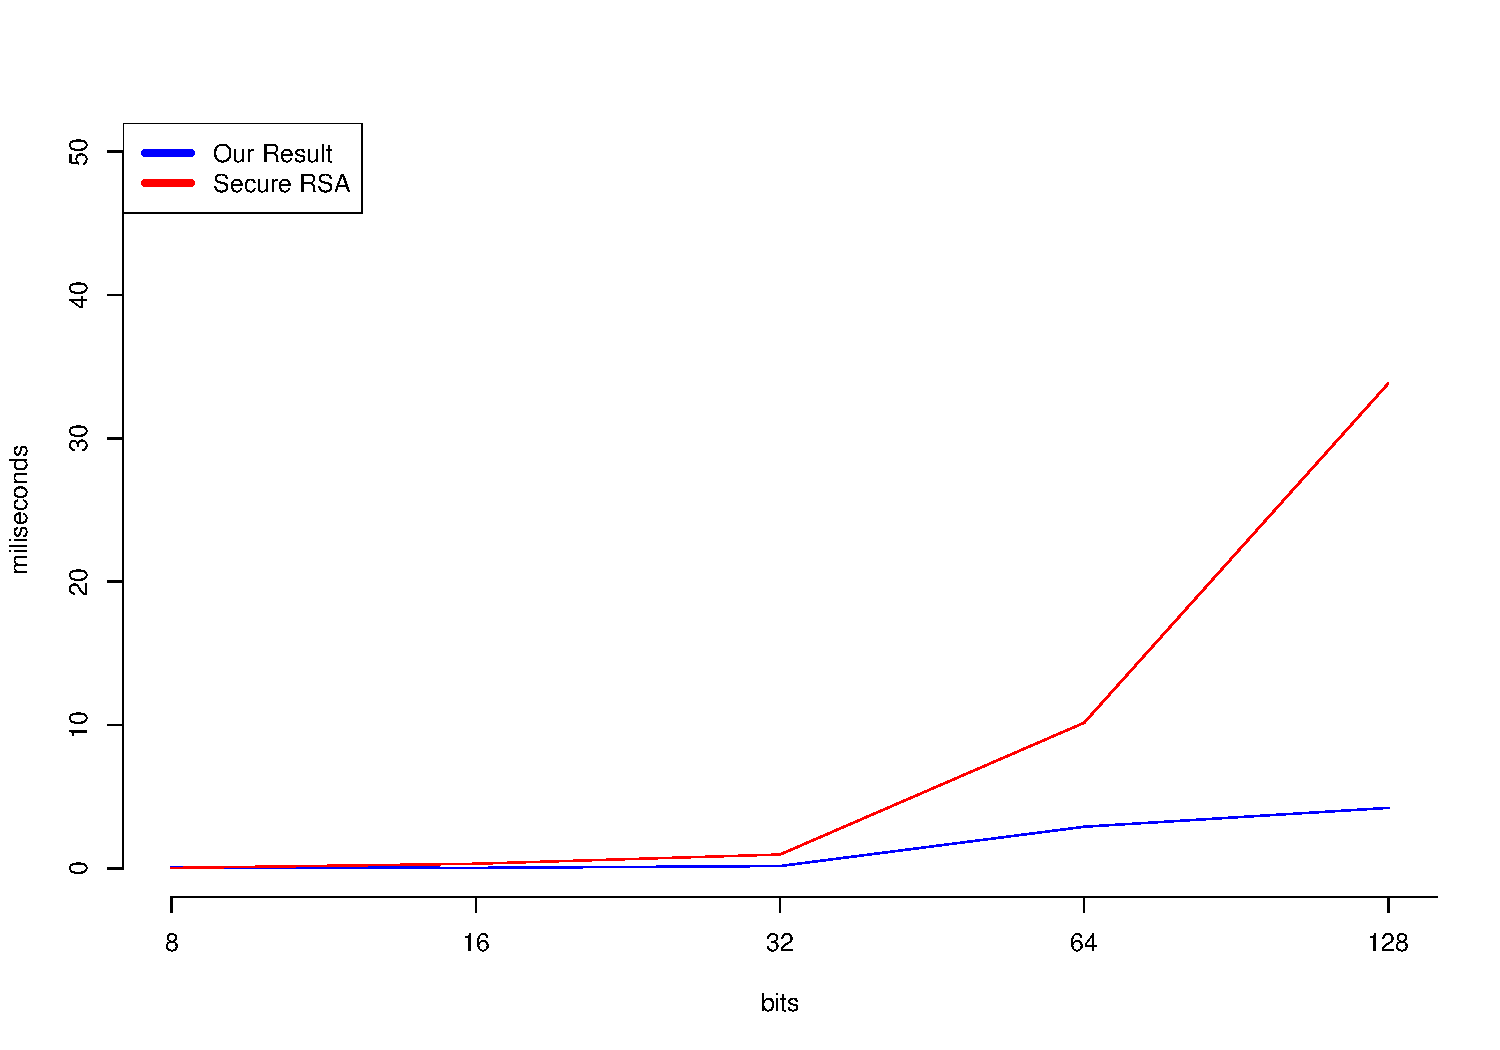
\includegraphics[width=90mm]{images/rsaVSjava.pdf}
\caption{Time comparison of performance}
\label{fig:rsaVSjava}
\end{figure}


Secure RSA as defined in Section \ref{sec:mrea_algo} needs large multiplicative computation for large prime numbers which will take $O(n^2)$ digit operation thus limiting the performance. To overcome this we needed faster algorithm for multiplication which we are going to explain in the next section.

%KARATSUBA MULTIPLICATION
\subsection{{Karatsuba Multiplication}}
\label{sec: karatsuba_code}
Karatsuba's algorithm for fast multiplication was first published in "\emph{Multiplication of Many-Digital Numbers by Automatic Computers}"\cite{karatsuba}, Proceedings of the USSR Academy of Sciences. The algorithm space for this algorithm is surprisingly rich. There are many methods of integer multiplication beyond what we learnt called conventional long multiplication and this is one of them. 

\subsubsection{\bf Mathematical Derivation}

To illustrate the algorithm, we let $X$ and $Y$ be two $2k$-bit unsigned integer and split them both in half
\begin{align}
X &= 2^{k}X_{1} + X_{0} \notag \\
Y &= 2^{k}Y_{1} + Y_{0} 
\end{align}
In conventional long multiplication, the product $XY$ is computed with four $k$-bit multiplications and three additions as shown in Equation \ref{eq:eq0}

\begin{align}
\label{eq:eq0}
XY &= 2^{2k}z_{2} + 2^{k}z_{1} + z_{0}
\end{align}

\begin{align}
\label{eq:eq1}
z_2 = X_{1}Y_{1}, z_{1} = X_{0}Y_{1} + X_{1}Y_{0}, z_{0} = X_{0}Y_{0}
\end{align}

As shown in Equation \ref{eq:eq1}, Karatsuba\cite{karatsuba} noticed that the middle term $z_1$ can be computed reusing the terms $z_2$ and $z_0$. Reusing these terms allow us to  replace two of the multiplications and one addition with four additions/subtractions and one multiplication

\begin{align}
z_{1} &=  X_{0}Y_{1} + X_{1}Y_{0} \notag\\
&=  X_{1}Y_{1} + X_{0}Y_{0} - (X_{1} - X_{0})(Y_{1} - Y_{0}) \notag\\
XY &= T_{1} - T_{2} \notag \\
T_{1} &= 2^{2k}z_{2} + z_{0} + 2^{k}(z_{2} + z_{0}) \notag \\
T_{2} &= 2^{2k}(X_{1} - X_{0})((Y_{1}-Y_{0})
\label{eq:eq2}
\end{align}


To elaborate, let's take an example of $x = 5678 \text{ and } y = 1234$. Now we will split first number $x$ into two halves as $a=56 \text{ and }b=78$ similarly for $y$, $c=12 \text{ and } d=34$

\begin{enumerate}[ {STEP }1{:} ]
	\item Compute $a \times c = 672$
	\item Compute $b \times d = 2652$
	\item Compute sum of $(a + b)\times (c +d) = 134 \times 46 = 6164$
	\item Compute STEP 3 - STEP 2 - STEP 1 = 2840
	\item Pad result of STEP1 with 4 zeros, pad 2 zeros for result from STEP 4 and add them along with result from STEP 2 and resultant is the required result which is 7006652.
\end{enumerate}

Also, Xin  and Ziaofei\cite{378085} analysed the critical techniques that may be combined in the design of fast hardware for RSA cryptography: Chinese remainders, star chains, Hensel's odd division (also known as Montgomery modular reduction), carry-save representation, quotient pipelining, and asynchronous carry completion adders.

Assuming that we replace two of the multiplications with only one makes the program faster. The question is how fast? Using Karatsuba, we improved the multiplication process by replacing the initial complexity of $O(n^{2})$ by $O(n^{\log 3})$, which can be seen in the Figure \ref{fig:karatsubaVSgrade} for the performance of Karatsuba Multiplication over conventional multiplication for big n.

%\begin{figure}[ht!]
%\centering
%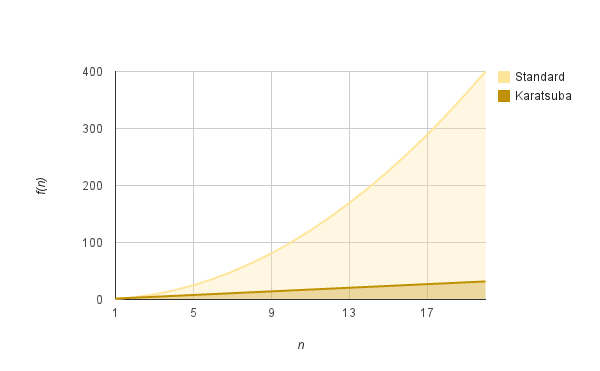
\includegraphics[width=90mm]{images/Karatsuba-Complexity.png}
%\caption{Karatsuba Multiplication Performance}
%\label{fig:karatsube_image}
%\end{figure}

\subsubsection{\bf Karatsuba Algorithm Implementation}

The algorithm we followed to generate result for Karatsuba multiplication is explained in Algorithm \ref{alg_karatsuba}
\begin{algorithm}                      % enter the algorithm environmen\LARGEt
\caption{Karatsuba Multiplication}          % give the algorithm a caption
\label{alg_karatsuba}                           % and a label for \ref{} commands later in the document
\begin{algorithmic}                    % enter the algorithmic environment
    \REQUIRE two large numbers $n_1$ and $n_2$
    \ENSURE product of $n_1$ and $n_2$

   %\STATE Function($n_1$, $n_2$)
    \IF{$n_1 < 10$ \OR $n_1 < 10$}
    	\RETURN{$n_1 \times n_2$}
    \ENDIF
    
    \IF{$n_1 > n_2$}
    	\STATE{$m = n_1$}
    \ELSE
    	\STATE{$m = n_2$}
    \ENDIF
    
    \STATE{$m_2 = \frac{m}{2}$}
    
    \COMMENT{split the digit sequences about the middle}
    \STATE{$high_1, low_1 = split\_at(n_1, m_2)$}
    \STATE{$high_2, low_2 = split\_at(n_2, m_2)$}
    
    \STATE{$z_0 = karatsuba(low_1, low_2)$}
    \STATE{$z_1 = karatsuba((low_1+high_1), (low_2+high_2))$}
    \STATE{$z_0 = karatsuba(high_1, high_2)$}
    \RETURN{$(z_2 \times 10^{2 \times m_2})+ ((z_1 - z_2 - z_0)\times 10^{m_2})+(z_0)$}
\end{algorithmic}
\end{algorithm}
%\parbox{\linewidth}{
%	\lstinputlisting[label = samplecode, firstline=195,lastline=232]{RSA.py}
%}

We measured the program and found the results of multiplication for pairs of random \emph{n}-digit numbers which is in TABLE \ref{table:karatsubaVSgrade} and Figure \ref{fig:karatsubaVSgrade}. All times are in milliseconds and  shows results we obtained.

To increase the security of encryption we need pseudorandom number generator with large period. To achieve so Linear Congruential Generator (LCG)\cite{lcg_cryptography} can be used which is fast and require minimal memory (typically 32 or 64 bits) to retain state. This makes them valuable for simulating multiple independent streams but it is not recommended where high-quality randomness is critical which is highly prioritized in cryptography. If a linear congruential generator is seeded with a character and then iterated once, the result is simple classical cipher called an affine cipher\cite{affine_cipher}; this cipher is easily broken by standard frequency analysis. Also, LCG tend to exhibit some severe defects. for instance, if a LCG is used to choose points in $n$-dimensional space, the points will lie on, at most $m^{\frac{1}{m}}$ hyperplanes\cite{marsaglia_theorem}. For this research, we introduced Mersenne Twister (MT19937) pseudorandom number generator which we will explain in next section.


\begin{table}[ht]
	\begin{center}
	\begin{tabular}{|c|c|c|}
    	\hline
       		digits 	&		Karatsuba					&	Long Conventional Multiplication\\
	\hline
    		8		&		0.059923					&	0.063902 \\
		16		&		0.006230					&	0.006141 \\
		32		&		0.016622					&	0.017437 \\
		64		&		0.048354					&	0.058411 \\
		128		&		0.140272					&	0.212314 \\
		256		&		0.437445					&	0.808407 \\
		512		&		1.317523					&	3.164557 \\
	\hline
	\end{tabular}
	\end{center}
	\caption{Karatsube VS Long Conventional Multiplication Time}
	\label{table:karatsubaVSgrade}

\end{table}

\begin{figure}[ht!]
\centering
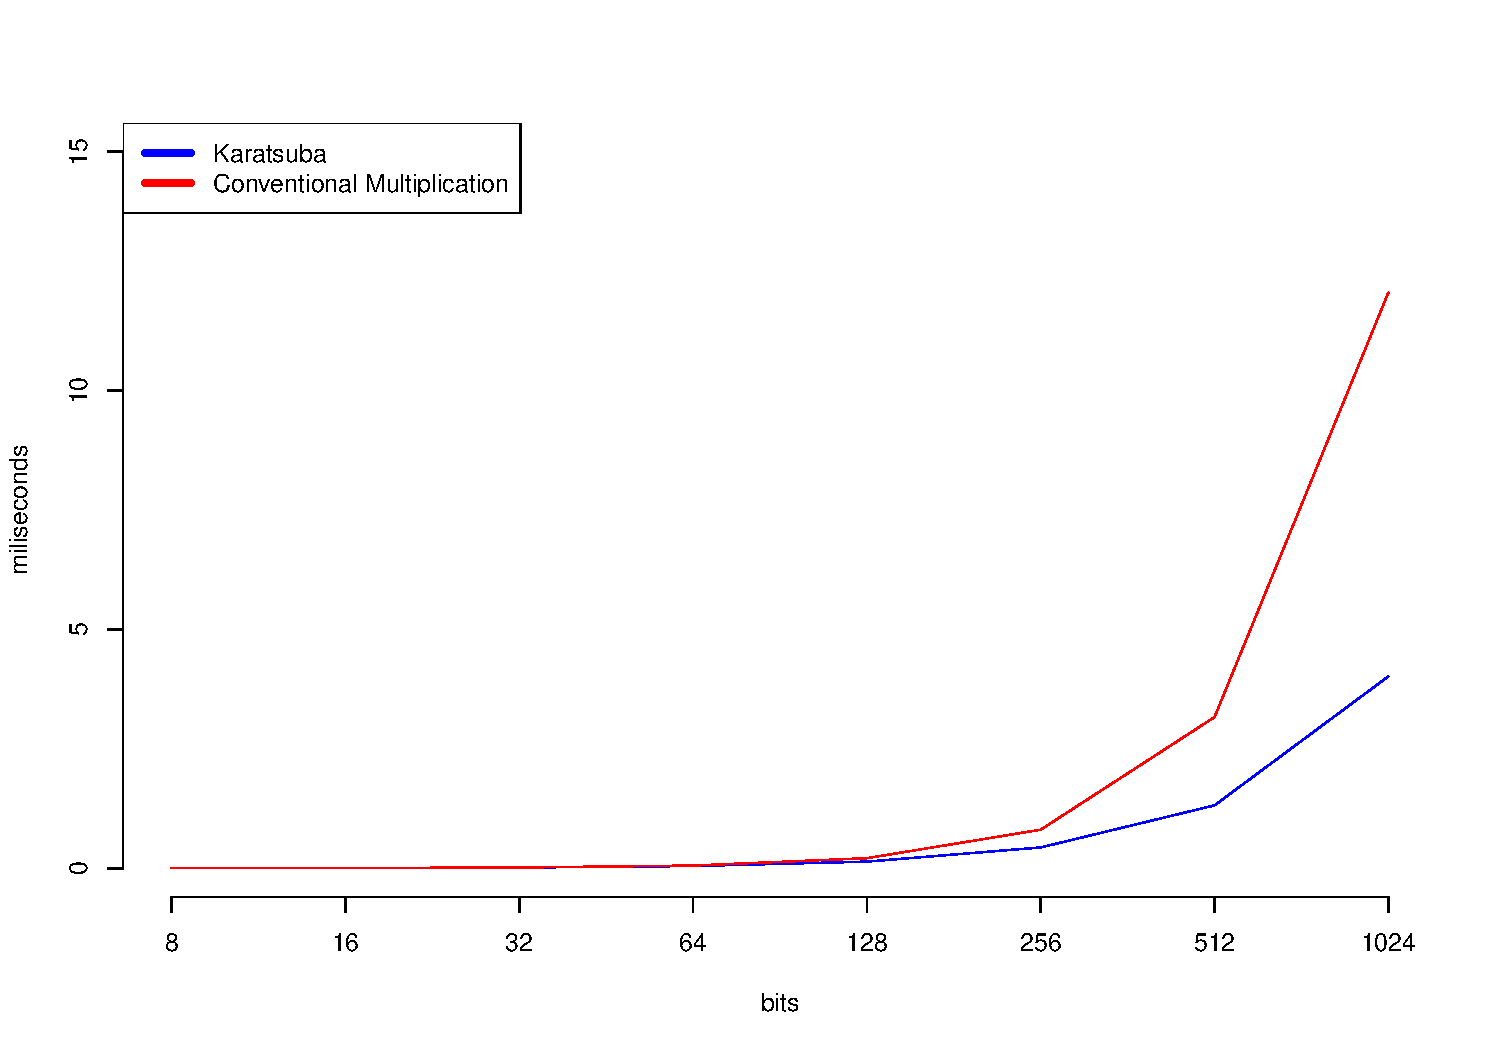
\includegraphics[width=90mm]{images/karatsubaVSgradeSchool.pdf}
\caption{Graph of results for Karatsuba and Grade School Multiplication}
\label{fig:karatsubaVSgrade}
\end{figure}


%MERSENNE PRIME
\subsection{{Pseudorandom Number Generation}}
\label{sec:mersenne}
The Mersenne twister\cite{MT19937} is pseudorandom number generator. It is, by far, the most widely used Pseudorandom number generator. It's name derives from the fact that it's period length is chosen to be 24\textsuperscript{th} Mersenne Prime though the "guarantee" isn't there anymore. MT19937 is a variant of the twisted generalised feedback shift-register algorithm. It has passed the DIEHARD statistical tests. MT19937 uses 624 words of state per generator and is comparable in speed to the other generators. The original generator used a default seed of 4357 and "choosing \emph{{\bf s}} equal to zero".\cite{MT19937}

 It is quite possible to have a random generator that produces the exactly same values for two different seeds. This isn't an issue unless we depend on some behavior of the randomness. The main point of course being cryptography is crypto graphical random number generators try very hard to be very random even if we run 10 generators in parallel. However, this might defeats the purpose of repeatability. The authors claim speeds 1.5 to 2 times faster than \emph{Advanced Encryption Standard in counter mode}\cite{1347044}.

\begin{figure}[ht!]
\centering
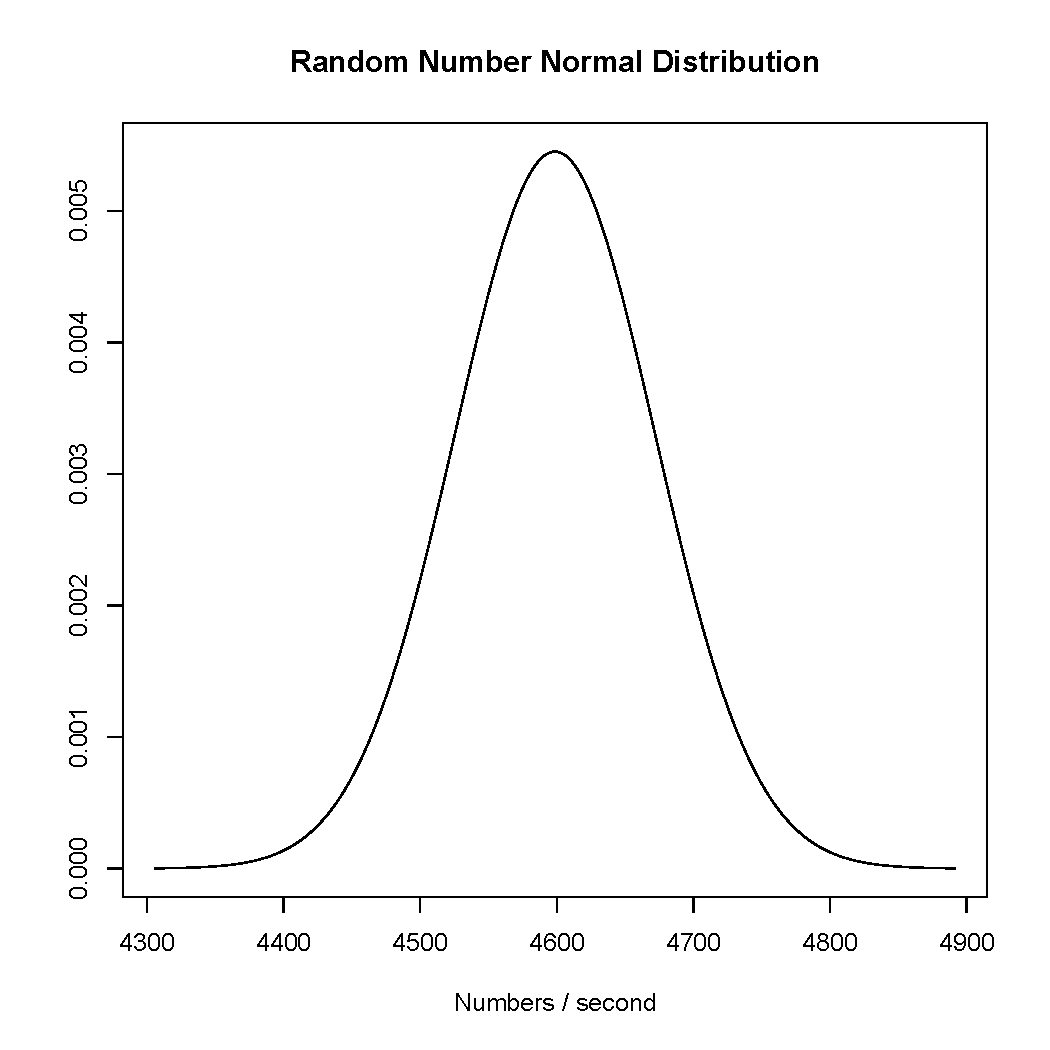
\includegraphics[width=90mm]{images/plotRandomNumber.pdf}
\caption{Normal Distribution of Random Number Generator}
\label{fig:plotRandomNumber}
\end{figure}
 
 %The MT19937 algorithm is inherently 32-bit, but works nicely on 64-bit systems. While it uses the all 32 bits to express pseudo-random numbers, rand() does not. By design it will only return numbers in the range 0 ... INT32\_MAX, effectively using only 31 bits of randomness. This is a well known point of criticism for rand(). This assumes that the compiler is using two's complement for encoding negative numbers.
 
The MT19937 generates sequence of word vectors, which are considered uniform pseudorandom integers between $0$ and $(2^{w}-1)$\cite{MT19937}. Dividing by $2^{w}-1$, each word vector can be a real number in $[0, 1]$. With the restriction that $2^{nw-r}-1$ is a Mersenne prime. For a word $x$ with $w$ bit width, it is expressed as the recurrence relation:
\begin{equation}
\label{eq:mersenne_recc}
x_{k+n} =  x_{k+m} \oplus (x^{u}_{k} | x^{l}_{k+1})A; k=0,1,2.....
\end{equation}
In Equation \ref{eq:mersenne_recc} $|$ represent as the bitwise OR and $\oplus$ represent as the bitwise exclusive or XOR, $x_w, x_l$ being $x$ with upper and lower bit masks applied. We choose a form of a matrix $A$ so that multiplication by $A$ is very fast:
\begin{align}
A = R = \begin{pmatrix} 0 & I_{w-1} \\ a_{w-1} & (a_{w-2},.....a_{0}) \end{pmatrix} 
\end{align}
With $I_{n-1}$ as the $(n-1) \times (n-1)$ identity matrix (and in contrast to normal matrix multiplication, bitwise XOR replaces addition). The rational normal form has the benefit that it can be efficiently expressed as:
\begin{align}
xA = \begin{cases}
	ShiftRight(x), & \text{if $x_0 = 0$}.\\
    	ShifrRight(x)\oplus a, & \text{if $x_{0} = 1$}.
	\end{cases}
\end{align}
Where
\begin{align}
x = (x^{u}_{k} | x^{l}_{k+1}); k = 0, 1, 2, .....
\end{align}
and
\begin{align*}
a &= (a_{w-1}, a_{w-2}, ......, a_{0}) \\
%x &= (x_{w-1}, x_{w-2}, ......, x_{0})
\end{align*}


To improve $k$-distribution to $v$-bit accuracy, we multiply each generated word by a suitable $w \times w$ invertible matrix $T$ from the right. For the tempering $r \rightarrow z = xT$, we chose the following successive transformations:
\begin{align}
y &= x \oplus (x>>u) \\
y &= x \oplus (x<<s) \text{ AND } b \\
y &= x \oplus (y << t) \text{ AND } c \\
y &= x \oplus (x >> l)
\end{align}
With $<< \text{ and }>>$ as the bitwise left and right shifts and $\&$ as the bitwise AND. The first and last transforms are added in order to improve lower bit equidistribution. From the property of TGFSR, $s+t \geq \lfloor \frac{w}{2}\rfloor -1$ is required to reach the upper bound of equidistribution for the upper bits. \\*
According to MT19937\cite{MT19937} The coefficients are:
\begin{align}
(w,n,m,r) &= (32, 624, 397, 31) \notag \\
a &= 9908B0DF_{16} \notag\\
u &= 11 \notag \\
(s, b) &= (7, 9D2C5680_{16}) \notag \\
(t, c) &= (15, EFC60000_{16}) \notag \\
l &= 18
\label{eq:mersenne_table_values}
\end{align}
The algorithm for Equation \ref{eq:mersenne_recc} through Equation \ref{eq:mersenne_table_values} can be summarized in Algorithm \ref{alg_mersenne_twister} which is derived from "\emph{Mersenne Twister: A 623-dimensionally equidistributed uniform pseudorndom number generator}"\cite{MT19937} The values for parameters $w, n, m, r, a, u, s, b, t, c \text{ and }l$ are taken from \emph{Table $II$ Parameters and k-distribution of Mersenne Twisters}\cite{MT19937}. .

\begin{algorithm}                      % enter the algorithm environment
\caption{Mersenne-Twister}
\label{alg_mersenne_twister}                           % and a label for \ref{} commands later in the document
\begin{algorithmic}                    % enter the algorithmic environment
   %\REQUIRE $n>2$, an odd integer to be tested for primality; $k$, a parameter that determines the accuracy of the test
    
    %\ENSURE composite if $n$ is composite, otherwise probably prime.
    
    \STATE {\bf Step0: } \\
    $u \leftarrow \underbrace{1...1}_{w-r}\underbrace{0...0}_{r}; (\text{ bitmask of upper w-r})$ \\ 
    $ll \leftarrow \underbrace{1...1}_{w-r}\underbrace{0...0}_{r}; (\text{ bitmask of lower r bits})$ \\
    $a \leftarrow a_{w-1}a_{w-2}a_{w-3}...a_{2}a_{1}$
    
    \STATE {\bf Step1: }\\
    $i \leftarrow 0$ \\
    $x[0], x[1], x[2].....x[n-1]\leftarrow \text{ "any non-zero initial values"}$
    
    \STATE {\bf Step2: }\\
    $y \leftarrow (x[i] \text{ AND }u) \text{ OR } (x[(i+1) \mod n] \text{ AND }ll)$ \\
    
    \STATE {\bf Step3: }
    $x[i] \leftarrow x[(i+m) \mod n] \text{ XOR } (y>>1)$ \\
    	$
		\text{ XOR } \begin{cases}
					0, & \text{if least significant bit of y=0}.\\
    					a, & \text{if least significant bit of y = 1}.
				\end{cases}
    	$
    
    \STATE {\bf Step4: } calculate $x[i]T$ \\ 
    \begin{align*}
    	y &\leftarrow x[i]\\
	y &\leftarrow y \text{ XOR } (y>>u) \\
	y &\leftarrow y \text{ XOR } ((y<<s) \text{ AND } b) \\
	y &\leftarrow y \text{ XOR } ((y << t) \text{ AND } c) \\
	y &\leftarrow y \text{ XOR } (y >> l)
\end{align*}
    
    \STATE {\bf Step5: } \\
    \begin{align*}
    	i \leftarrow (i+1) \mod n
    \end{align*}
    
    \STATE {\bf Step6: }Goto {\bf Step2}
\end{algorithmic}
\end{algorithm}
Also, the authors of MT19937\cite{MT19937} mentioned for Equation \ref{eq:mersenne_table_values} that "\emph{If $r=0$, then this recurrence reduces to the previous TGFSR}" which was the reason we included this version of algorithm in our work and change the value of $r$ to user's need.

Mersenne Twister implementations cannot be parallelized across parallel computing cores simply through changing the initial seed for each core as this does not provide uncorrelated sequences on each generator sharing identical parameters. To solve this problem and enable Mersenne twister parallel implementations, the authors of MT19937\cite{MT19937} developed a library for the dynamic creation of Mersenne Twister parameters. This library receives user's specification such as word length, period, size of working area and a process ID, so that ID number is encoded in the characteristic polynomial of Mersenne Twister.
\begin{figure}[ht!]
\centering
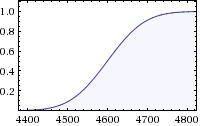
\includegraphics[width=90mm]{images/cdf_mersenne.jpeg}
\caption{Cumulative Density Function}
\label{fig:cdf_mersenne}
\end{figure}


Figure \ref{fig:cdf_mersenne} shows the Cummulative Density Function (which is defined by $F(x) = P(X\leq x)$) graph for the random number generator with mean of 4600 and standard deviation of almost 74. 


MT19937 we worked with showed the following statistical property which makes it preferable over other pseudorandom number generators.\cite{wolfram_mt}
\begin{itemize}
	\item {\bf Probability Density Function: }\\
		$0.00535134e^{-0.0000899652 (x-4599.84)^{2}}$
	\item {\bf Cumulative Distributive Function (CDF): }\\
		$\frac{1}{2}erfc(0.009485(4599.84-x))$
\end{itemize}

For faster primality test for random number generated by MT19937 we used Miller-Rabin Primality test which is by far fastest performing algorithm. We are going to explain the implementation in next section.

%MILLER-RABIN
\subsection{{Miller-Rabin Primality Test\cite{miller-rabin}}}
We know of two ways to prove that a number $n$ is composite:
\begin{enumerate}
\item Exhibit a factorization $n = ab$, where $a,b >1$
\item Exhibit a Fermat\cite{fermat} witness for $n$, \emph{i.e} a number $x$ satisfying $x^{n-1}\not\equiv 1 (\mod n)$
\end{enumerate}
The Miller-Rabin test is based on a third way to prove that a number is composite
\begin{enumerate}[ {}3{)} ]
\item Exhibit a "fake square root of $1 \mod n$" \emph{i.e} a number $x$ satisfying $x^{2} \equiv 1(\mod n)$ but $x \not \equiv \pm1 (\mod n)$
\end{enumerate}

If $x, n$ are positive integers such that $x^{2} \equiv 1 (\mod n)$ but not $x \not \equiv \pm1 (\mod n)$ then $n$ is composite. Generally this can be proved that for any nonzero polynomial
\begin{align}
P(x) = a_0 + a_1x + ... + a_kx^k \notag
\end{align}
The numder of $x \in {1, 2, 3, ... , p-1}$ satisfying $P(x) \equiv 0 (\mod p)$ is at most $k$. The proof is by induction on $k$, the base case $k = 0$ being trivial. Otherwise, suppose $a$ satisfies $P(a) \equiv 0 (\mod p)$. We may write $P(x) = (x - a)Q(x) + c$ where $Q(x)$ is a polynomial of degree $k-1$ with integer coefficients. The congruence $P(a) \equiv 0 (\mod p)$ implies that $c$ is divisible by $p$. If $b$ satisfies $P(b) \equiv 0 (mod p)$ but $Q(b) \not \equiv 0 (\mod p)$ then $p$ is a divisio of $(b-a)Q(b)$ but not $Q(b)$, hence $b \equiv a (mod p)$. It follows that every $b \in {1,2,3,...,p-1}$ satisfying $P(b) \equiv 0 (\mod p)$ satisfies either $b = a$ or $Q(b)\equiv 0(\mod p)$. By the induction hypothesis, at most $k-1$ elements of ${1, 2,...,p-1}$ satisfy the second congruence\cite{miller-rabin}
%The Miller-Rabin test is shown in Algorithm \ref{alga}. 

The idea of test is to pick a random $x$ in ${1,2,3,.....,n-1}$ and use it to try finding either a Fermat witness\cite{fermat} or a fake square root of $1 \mod n$. Why Miller-Rabin test works? We have seen that when $n$ is prime, the test always outputs "probably prime". When $n$ is composite but is not a \emph{Carmichael} number, we have seen that it outputs "composite" with probability at least $\frac{1}{2}$. The working on Miller-Rabin test in this case best be understood in terms of \emph{Chinese Remainder Theorem}\cite{chinese_theorem} which is;


"\emph{Let $n_1, n_2,...,n_k$ be numbers, no two of which have a common factor. For any numbers $a_1, a_2, a_3,...,a_k$, the system of congruences }
\begin{align*}
x &\equiv a_1 (\mod n_1) \\
x &\equiv a_2 (\mod n_2) \\
&.\\
&.\\
x &\equiv a_k (\mod n_k) \\
\end{align*}
\emph{has a solution. Any two solutions $x_1, x_2$ are congruent $\mod n_1 n_2 ... n_k$"}. If $n$ is a \emph{Carmichael} number, then Miller-Rabin outputs "composite" with probability at-least $\frac{3}{4}$. %By analogy with the definitions of Fermat Witness and Fermat Liar\cite{fermat}, let us call a number $x$ a "Miller-Rabin witness"


The Miller-Rabin can be summarized that the number to be tested say $p$ and $y$ be a non trivial square root of $1 (\mod p)$.\cite{miller-rabin} Then we must have that $y^{2} = 1 (\mod p)$ and so $(y-1)(y+1) = 0(\mod p)$. This implies that either $y = 1 \mod p$ or $y = -1 \mod p$, which implies that $y$ is a trivial square root.


\begin{algorithm}                      % enter the algorithm environment
\caption{Miller-Rabin Primality Algorithm}          % give the algorithm a caption
\label{alg1}                           % and a label for \ref{} commands later in the document
\begin{algorithmic}                    % enter the algorithmic environment
    \REQUIRE $n>2$, an odd integer to be tested for primality; $k$, a parameter that determines the accuracy of the test
    \ENSURE composite if $n$ is composite, otherwise probably prime.
    
   \STATE{write $n-1$ as $2^{s}d$ with $d$ odd by factoring powers of $2$ from $n-1$}
   
   \REPEAT
   	\STATE {$x \leftarrow a^{d} \mod n$}
	\IF{$x = 1$ \OR $x = n-1$}
		\STATE{continue}
	\ENDIF
	\FOR{$r = 1 to s-1$}
		\STATE{$x \leftarrow x^{2}\mod n$}
		\IF{$x = 1$}
			\RETURN{composite}
		\ENDIF
		\IF{$x = n-1$}
			\STATE{do next loop}
		\ENDIF
	\ENDFOR
	\RETURN{composite}
   \UNTIL{k times}
   \RETURN{probably prime}
\end{algorithmic}
\end{algorithm}

Thus, if there is a non trivial square root of $1 \mod p$, then $p$ has to composite. For an example of a non trivial square root of a composite, consider $p = 15$. We have that $4^{2} = 16 = 1 (\mod 15)$, thus 15 is composite. The fact about non trivial square roots can be used to prove that if $p$ is prime, then for any $a$ relatively prime to $p$, some power of $a$ from a given set of powers must be $-1$ or a specific odd power of $a$ must be $1$.


If for some $a$ none of the above set of powers is $-1$ and the specific odd power is not 1, then it must be the fact that p is composite. It can also be shown that for composite $p$, the chances of finding such $a$ is at least $\frac{3}{4}$. This $a$ is the witness in the primality test and is not necessarily a non-trivial square root of $1 \mod p$. The algorithm is defined in Algorithm \ref{alg1}


%\parbox{\linewidth}{
%	\lstinputlisting[label = samplecode, firstline=1,lastline=33]{miller_rabin.py}
%}
 
%RESULTS
\section{{Results}}


\subsection{{Encryption \& Decryption}}

Though, introduction to one more random prime number slowed the performance but using Karatsuba Multiplication as mentioned in Algorithm \ref{alg_karatsuba} over came the limitation. To prove this hypothesis we ran test of generation of 60 encryptions and decryptions (10 sets of file encryption and decryption with 32, 65, 94, 127, 160, 320 \emph{bits} size random prime numbers) and found the performance to be significant. The result is shown in Figure \ref{fig:rsa_time}. We performed Normal Distribution Function and found that on average probability of encryption and decryption of 500 files is very high as shown in Figure \ref{fig:rsa_cdf}.

\begin{figure}[ht!]
\centering
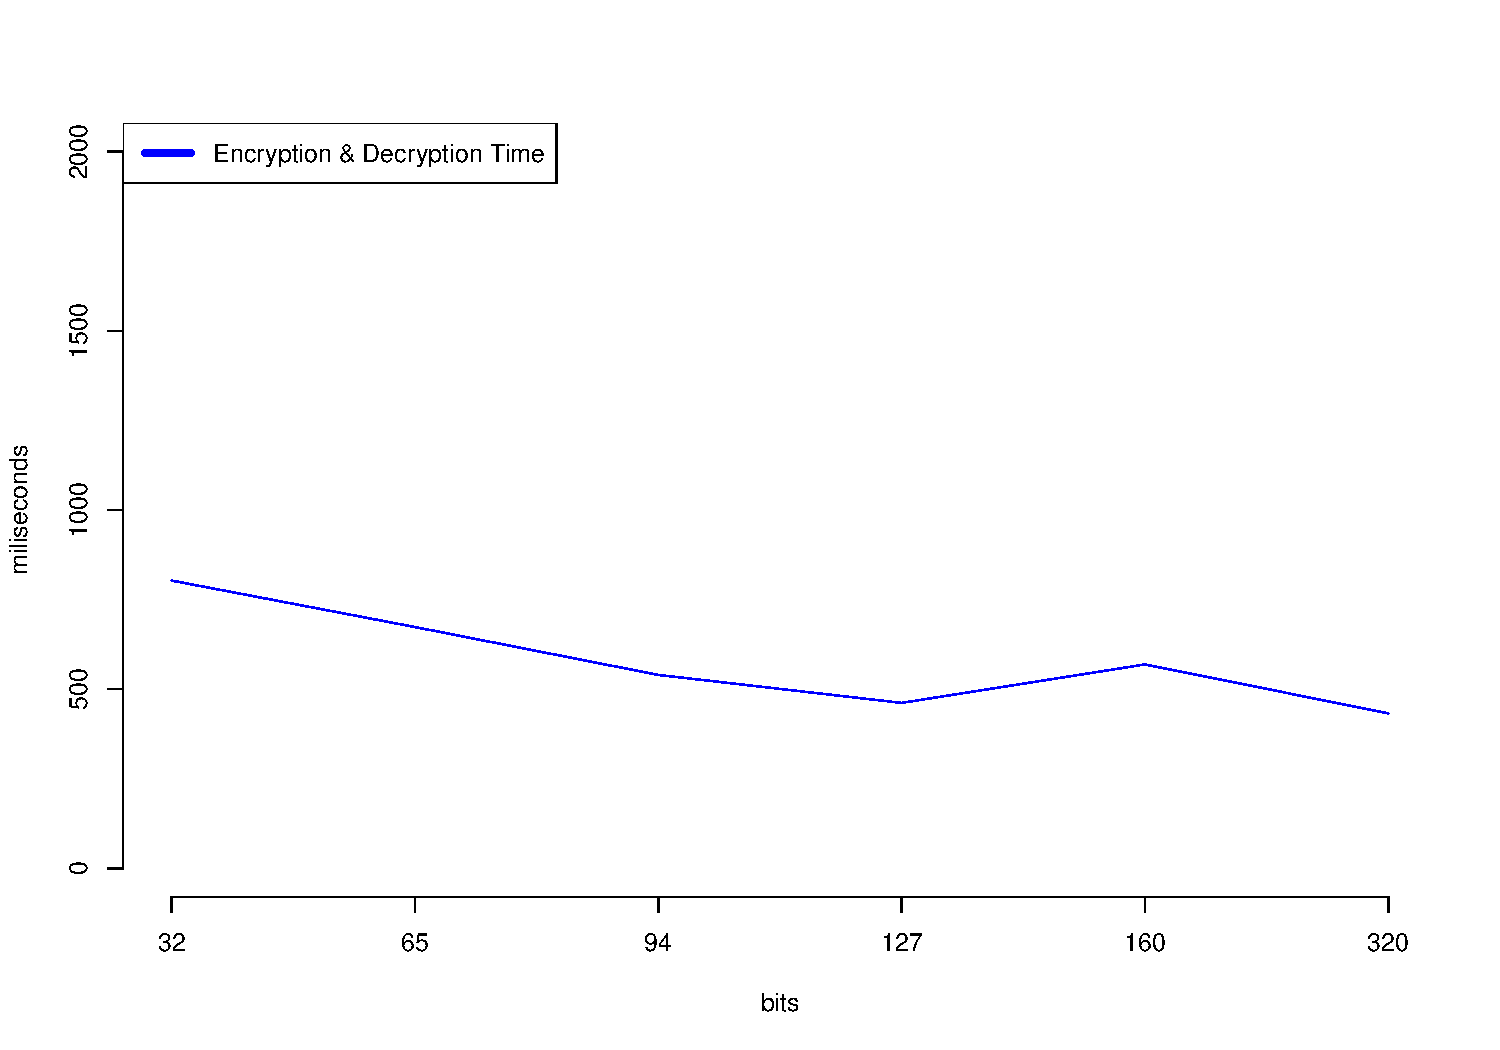
\includegraphics[width=90mm]{images/encryptionTime.pdf}
\caption{Encryption \& Decryption of file}
\label{fig:rsa_time}
\end{figure}

The algorithm have many important parameters affecting it's level of security and speed. By increasing the modulus length it is caused of increasing the complexity of decomposing it into it's factors. This also increases the length of private key and hence difficult to detect the key. Another parameter is modular multiplicative inverse $\mu$, which is new factor of private key, so it will be more difficult to choose $\mu$ by trying all possible private keys (brute force attack) hence the security also increases as well as difficulty of detecting the private key.


Furthermore, comparing this results with the "\emph{File Encryption and Decryption using Secure RSA}"\cite{securersa}, we found that our system had significant performance.


\begin{figure}[ht!]
\centering
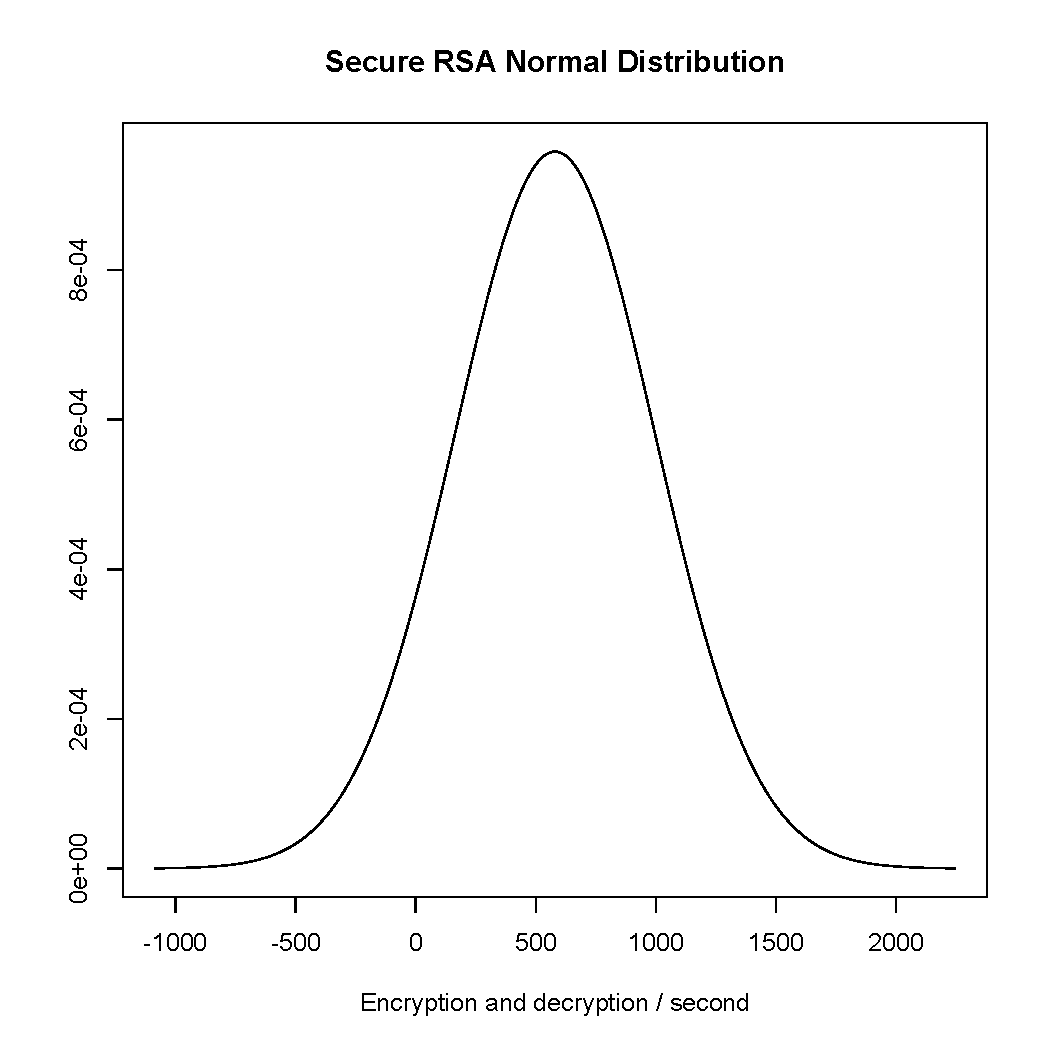
\includegraphics[width=90mm]{images/rsaPlot.pdf}
\caption{Normal distribution of Encryption \& Decryption of file}
\label{fig:rsa_cdf}
\end{figure}

\subsection{{Random Numbers}}
Our method for doing simple benchmarking and Mersenne Twister implementation generates numbers at a rate steadily over 4600 pseudo-random numbers per second which is very large. The test code reports normal distribution formulated from mean and standard deviation of performance of MT19937 is shown in Figure \ref{fig:mersenne_performance}.\cite{wolfram_mt}. Also, comparing our results with results mentioned in "Testing Random Number Generators"\cite{lcg_cdf} we found that as the number range increase the probability density increases exponentially (Figure \ref{fig:cdf_mersenne}) as compared to the results from paper\cite{lcg_cdf} which is linear and then remains constant. From this we can imply that as the key space of number increases probability density increases.

\begin{figure}[ht!]
\centering
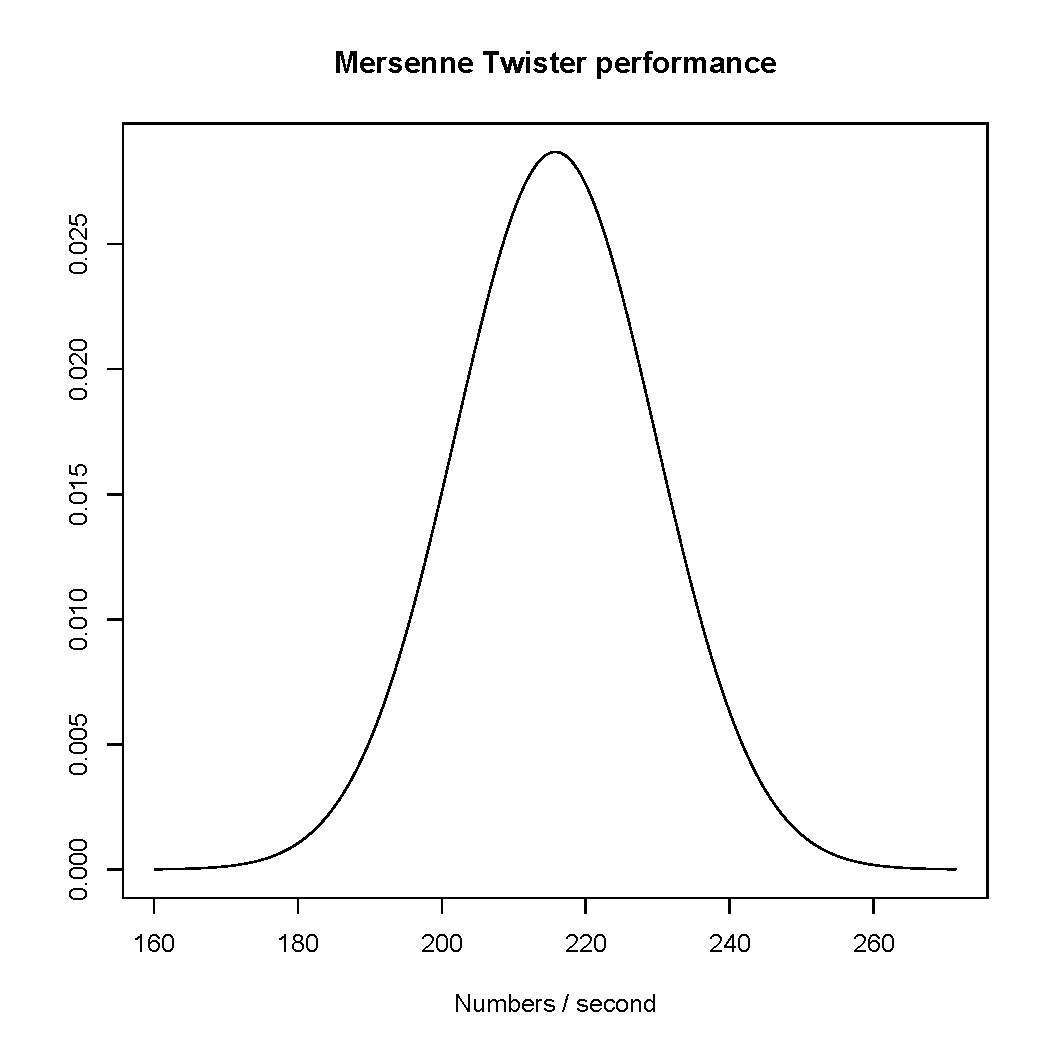
\includegraphics[width=90mm]{images/Rplot.pdf}
\caption{Mersenne Twister 19937 Performance}
\label{fig:mersenne_performance}
\end{figure}

Also, we tested to generate large prime number and our system showed significant performance to generate 34\textsuperscript{th} mersenne prime with negligible load on the system. Fig. \ref{fig:mersenne_time} shows the performance graph of the test conducted to compute time (in nano seconds) to generate large primes. To find the normal distribution for prime numbers generated using MT19937 we generated 31 sets of 100, 200, 300, 400, 500, 600 and 700 numbers. We found that on average our system is generating somewhat 216 random prime numbers per second with the standard of almost 14.

\begin{figure}[ht!]
\centering
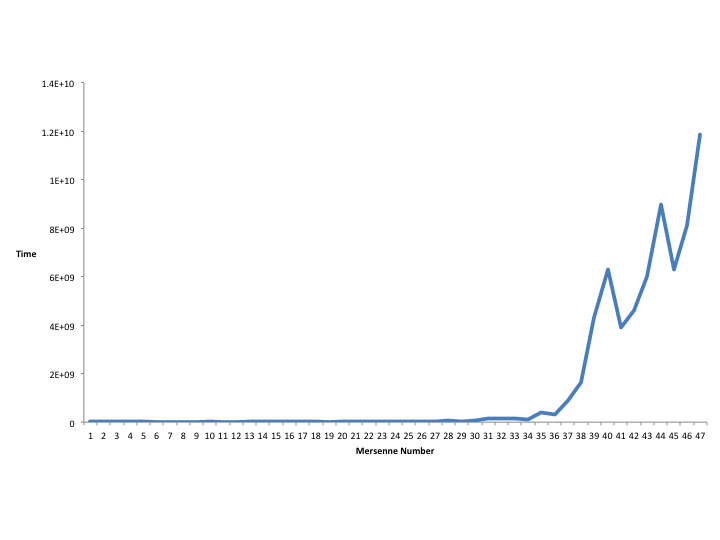
\includegraphics[width=90mm]{images/mersenneTime.png}
\caption{Time VS Mersenne Prime Number Generation}
\label{fig:mersenne_time}
\end{figure}
%Though GMPY2 is suitable for faster computation but it is limited to python's exponential computation. 


\subsection{{Large Multiplication}}
Karatsuba Multiplication\cite{karatsuba_multiplication} algorithm mentioned in section \ref{sec: karatsuba_code} was implemented to enhance the performance of multiplication also had significant performance as shown in Figure \ref{fig:karatsubaVSgrade}. The multipliers have significantly lower area-delay products compared with previous designs\cite{karatsuba_multiplication}. For key generation we worked to generate keys of size upto 512-bits to 1000-bits long keys for significant performance based on time of computation.

To further boost the multiplicative performance we used third party library for mathematical computation called GMPY2\cite{gmpy2} which is a Python module that provides access to the GNU Multiple Precision (GMP) library. GMP provides very fast and highly optimized routines for working with arbitrary precision integers, rationals, and floating point numbers.


\section{{Conclusion}}
The digital world of cryptography is getting bigger and bigger, not smaller and our method have showed a new approach to make secure by increasing the bit size of the key generated with not compromising with good computational performance up to 512-bit long keys and comparatively significant performance up to 1900-bit long key for encryption and decryption. 


Secure RSA algorithm is used to encrypt files and transmit encrypted files to other end where it is decrypted. Our system works on the large numbers. It has broad development prospects. The system application was designed to take the efficiency and reusability into account. Great level of security is achieved using this algorithm. Secure RSA algorithm for file transmission algorithm can be used where high security file transmission required in public forums.


With the increasing computing power available to even casual users, the security conscious have had to move on to increasingly robust encryption, lest they find their information vulnerable to brute-force attacks. The latest milestone to fall is 768-bit RSA. In "\emph{Factorization of a 768-bit RSA modulus}"\cite{768_key} announced that they factored one of these keys. 


Most modern cryptography relies on single large number that are the product of two primes. By knowing the numbers, it is relatively easy to encrypt and decrypt data, otherwise finding by brute force is big computational challenge. "\emph{There is nothing new to be reported for the square root step, except for the resulting factorization of RSA-768. Nevertheless, and for the record, we present some of the details}"\cite{768_key} they wrote.


As future work multiple file encryption and decryption can be possible. It has broad development prospects. 

{
\bibliographystyle{abbrv} %plain; ieeetr; alpha
\bibliography{ref}
}


% if have a single appendix: 
%\appendix[Proof of the Zonklar Equations]
% or
%\appendix  % for no appendix heading
% do not use \section anymore after \appendix, only \section*
% is possibly needed

% use appendices with more than one appendix
% then use \section to start each appendix
% you must declare a \section before using any
% \subsection or using \label (\appendices by itself
% starts a section numbered zero.)
%


%\appendices
%\section{Proof of the First Zonklar Equation}
%Appendix one text goes here.

% you can choose not to have a title for an appendix
% if you want by leaving the argument blank
%\section{}
%Appendix two text goes here.


% use section* for acknowledgement
%\section*{Acknowledgment}


%The authors would like to thank...


% Can use something like this to put references on a page
% by themselves when using endfloat and the captionsoff option.
%\ifCLASSOPTIONcaptionsoff
 % \newpage
%\fi



% trigger a \newpage just before the given reference
% number - used to balance the columns on the last page
% adjust value as needed - may need to be readjusted if
% the document is modified later
%\IEEEtriggeratref{8}
% The "triggered" command can be changed if desired:
%\IEEEtriggercmd{\enlargethispage{-5in}}

% references section

% can use a bibliography generated by BibTeX as a .bbl file
% BibTeX documentation can be easily obtained at:
% http://www.ctan.org/tex-archive/biblio/bibtex/contrib/doc/
% The IEEEtran BibTeX style support page is at:
% http://www.michaelshell.org/tex/ieeetran/bibtex/
%\bibliographystyle{IEEEtran}
% argument is your BibTeX string definitions and bibliography database(s)
%\bibliography{IEEEabrv,../bib/paper}
%
% <OR> manually copy in the resultant .bbl file
% set second argument of \begin to the number of references
% (used to reserve space for the reference number labels box)
%\begin{thebibliography}{1}

%\bibitem{IEEEhowto:kopka}
%H.~Kopka and P.~W. Daly, \emph{A Guide to \LaTeX}, 3rd~ed.\hskip 1em plus
%  0.5em minus 0.4em\relax Harlow, England: Addison-Wesley, 1999.

%\end{thebibliography}

% biography section
% 
% If you have an EPS/PDF photo (graphicx package needed) extra braces are
% needed around the contents of the optional argument to biography to prevent
% the LaTeX parser from getting confused when it sees the complicated
% \includegraphics command within an optional argument. (You could create
% your own custom macro containing the \includegraphics command to make things
% simpler here.)
%\begin{biography}[{\includegraphics[width=1in,height=1.25in,clip,keepaspectratio]{mshell}}]{Michael Shell}
% or if you just want to reserve a space for a photo:

%\begin{IEEEbiography}{Michael Shell}
%Biography text here.
%\end{IEEEbiography}

% if you will not have a photo at all:
%\begin{IEEEbiographynophoto}{John Doe}
%Biography text here.
%\end{IEEEbiographynophoto}

% insert where needed to balance the two columns on the last page with
% biographies
%\newpage

%\begin{IEEEbiographynophoto}{Jane Doe}
%Biography text here.
%\end{IEEEbiographynophoto}

% You can push biographies down or up by placing
% a \vfill before or after them. The appropriate
% use of \vfill depends on what kind of text is
% on the last page and whether or not the columns
% are being equalized.

%\vfill

% Can be used to pull up biographies so that the bottom of the last one
% is flush with the other column.
%\enlargethispage{-5in}



% that's all folks
\end{document}


